% Options for packages loaded elsewhere
\PassOptionsToPackage{unicode}{hyperref}
\PassOptionsToPackage{hyphens}{url}
%
\documentclass[
  12pt,
]{article}
\usepackage{amsmath,amssymb}
\usepackage{setspace}
\usepackage{iftex}
\ifPDFTeX
  \usepackage[T1]{fontenc}
  \usepackage[utf8]{inputenc}
  \usepackage{textcomp} % provide euro and other symbols
\else % if luatex or xetex
  \usepackage{unicode-math} % this also loads fontspec
  \defaultfontfeatures{Scale=MatchLowercase}
  \defaultfontfeatures[\rmfamily]{Ligatures=TeX,Scale=1}
\fi
\usepackage{lmodern}
\ifPDFTeX\else
  % xetex/luatex font selection
  \setmainfont[]{Times New Roman}
\fi
% Use upquote if available, for straight quotes in verbatim environments
\IfFileExists{upquote.sty}{\usepackage{upquote}}{}
\IfFileExists{microtype.sty}{% use microtype if available
  \usepackage[]{microtype}
  \UseMicrotypeSet[protrusion]{basicmath} % disable protrusion for tt fonts
}{}
\makeatletter
\@ifundefined{KOMAClassName}{% if non-KOMA class
  \IfFileExists{parskip.sty}{%
    \usepackage{parskip}
  }{% else
    \setlength{\parindent}{0pt}
    \setlength{\parskip}{6pt plus 2pt minus 1pt}}
}{% if KOMA class
  \KOMAoptions{parskip=half}}
\makeatother
\usepackage{xcolor}
\usepackage[margin=1in]{geometry}
\usepackage{longtable,booktabs,array}
\usepackage{calc} % for calculating minipage widths
% Correct order of tables after \paragraph or \subparagraph
\usepackage{etoolbox}
\makeatletter
\patchcmd\longtable{\par}{\if@noskipsec\mbox{}\fi\par}{}{}
\makeatother
% Allow footnotes in longtable head/foot
\IfFileExists{footnotehyper.sty}{\usepackage{footnotehyper}}{\usepackage{footnote}}
\makesavenoteenv{longtable}
\usepackage{graphicx}
\makeatletter
\def\maxwidth{\ifdim\Gin@nat@width>\linewidth\linewidth\else\Gin@nat@width\fi}
\def\maxheight{\ifdim\Gin@nat@height>\textheight\textheight\else\Gin@nat@height\fi}
\makeatother
% Scale images if necessary, so that they will not overflow the page
% margins by default, and it is still possible to overwrite the defaults
% using explicit options in \includegraphics[width, height, ...]{}
\setkeys{Gin}{width=\maxwidth,height=\maxheight,keepaspectratio}
% Set default figure placement to htbp
\makeatletter
\def\fps@figure{htbp}
\makeatother
\setlength{\emergencystretch}{3em} % prevent overfull lines
\providecommand{\tightlist}{%
  \setlength{\itemsep}{0pt}\setlength{\parskip}{0pt}}
\setcounter{secnumdepth}{-\maxdimen} % remove section numbering
\usepackage{booktabs}
\usepackage{longtable}
\usepackage{array}
\usepackage{multirow}
\usepackage{wrapfig}
\usepackage{float}
\usepackage{colortbl}
\usepackage{pdflscape}
\usepackage{tabu}
\usepackage{threeparttable}
\usepackage{threeparttablex}
\usepackage[normalem]{ulem}
\usepackage{makecell}
\usepackage{xcolor}
\ifLuaTeX
  \usepackage{selnolig}  % disable illegal ligatures
\fi
\usepackage{bookmark}
\IfFileExists{xurl.sty}{\usepackage{xurl}}{} % add URL line breaks if available
\urlstyle{same}
\hypersetup{
  pdftitle={Exploring the Impact of the Plus Program in Airbnb Performance},
  pdfauthor={Ana Ferreira, Claudius Kroflin, Edet Bassey, Federico Scandizzo},
  hidelinks,
  pdfcreator={LaTeX via pandoc}}

\title{Exploring the Impact of the Plus Program in Airbnb Performance}
\author{Ana Ferreira, Claudius Kroflin, Edet Bassey, Federico Scandizzo}
\date{}

\begin{document}
\maketitle

\setstretch{1.5}
\begin{figure}[h]
  \centering
  
\includegraphics[width=0.45\textwidth, height=2.5cm]{airbnb.png} 
  \hspace{0.75cm} 
  
\includegraphics[width=0.45\textwidth, height=2.5cm]{catolica.png} 
\end{figure}

\section{Introduction}\label{introduction}

In 2018, Airbnb introduced the Plus program, an initiative designed to
improve match-making for users seeking premium accommodations. The core
objective of this study is to evaluate the impact of the program and
determine whether differentiating high-quality services contributes to
improved platform performance.

The research will be structured by first providing a dataset overview,
outlining the relevant performance metrics, explanatory and other
secondary variables. Next, a data quality assessment is given by
explaining how missing values, inconsistencies and outliers were dealt
with. The exploratory data analysis comes next, starting with the
evolution of performance metrics overtime, highlighting the two
implementation dates of the Airbnb Plus program to emphasize before and
after changes.

The primary research question guiding this analysis is: ``What is the
impact of Airbnb Plus? Specifically, does distinguishing high-quality
services lead to enhanced platform performance?''

\newpage

\section{1. Dataset Overview}\label{dataset-overview}

The Dataset has a total of 14604 observations across 99 variables. It
covers 773 zipcodes within 11 US cities from the beginning of August
2017 (\texttt{timperiod} = 8) to the end of October 2019
(\texttt{timperiod} = 34).

The Airbnb Plus Program was only implemented in 5 cities, such as
\emph{San Francisco}, \emph{Denver}, \emph{Nashville}, \emph{New
Orleans} and \emph{Washington DC}. San Francisco got the program
implemented in February 2018 (\texttt{timeperiod\ =\ 14}) while the
others had it starting in October 2018 (\texttt{timeperiod\ =\ 22}).

For the scope of the research, the relevant key variables are the
following:

\begin{itemize}
\tightlist
\item
  \textbf{Performance Metrics:} \texttt{total\_bookings},
  \texttt{booking\_rate}, \texttt{listing\_avg\_review},
  \texttt{average\_booked\_nights}
\item
  \textbf{Secondary variables:} \texttt{zipcode}, \texttt{timeperiod},
  \texttt{city\_number}, \texttt{policy\_entry}
\end{itemize}

Other than the above, two new variables were created and added to the
data set:

\begin{itemize}
\tightlist
\item
  \textbf{\texttt{city\_name}}: transforms the \texttt{city\_number} to
  the name of the city according to the \texttt{zipcode}s included in it
  for relevant cities and to \emph{Others} for those who did not had the
  plus program introduced at any point in time
\item
  \textbf{\texttt{date}}: transforms the \texttt{timeperiod} into the
  correspondent \emph{year-month} format
\end{itemize}

\newpage

\section{2. Data Quality Assessment}\label{data-quality-assessment}

To assess the quality of the dataset, it is important to look at the
distribution of the key identified variables.

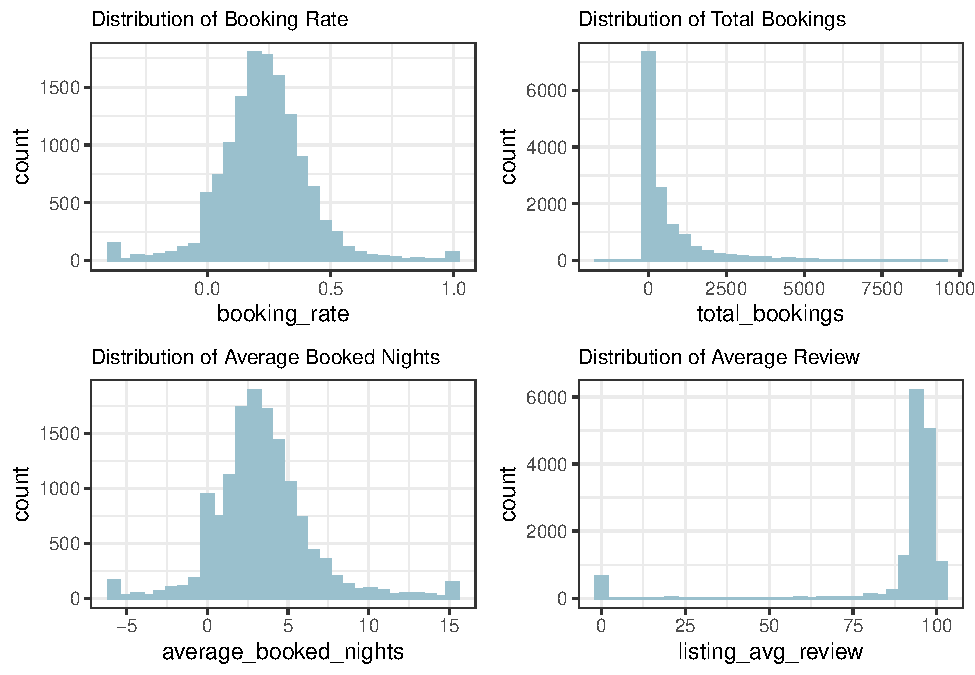
\includegraphics{Group-D---Assignment-1_files/figure-latex/unnamed-chunk-3-1.pdf}

The variables \texttt{booking\_rate} and
\texttt{average\_booked\_nights} have both negative to positive values.
When cancellations outweigh the bookings, the observation is a negative
value, and vice-versa. In the \texttt{listing\_avg\_review} there are
some ``0'' values, which affect the mean and distribution of this
variable. Given that Airbnb review ranges on a scale from 1 to 5 stars,
the 0 values will be treated the same as missing values (described later
in the section). Other than the above, it seems like there is no other
significant presence of outliers. To further investigate the variables,
a box plot distribution is shown for each one.

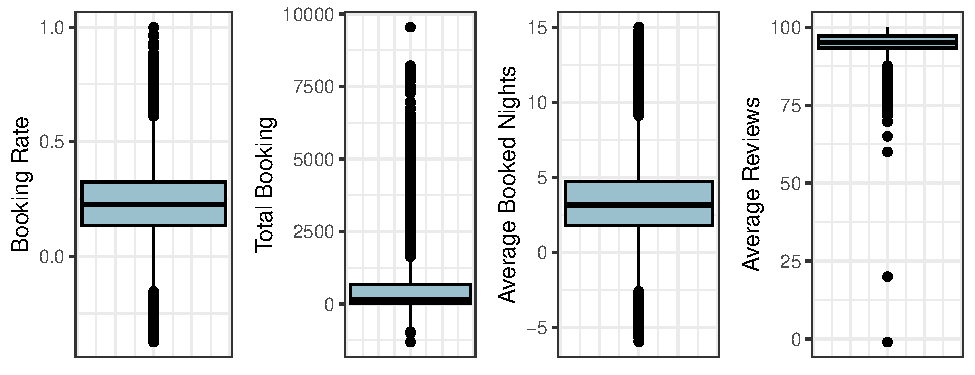
\includegraphics{Group-D---Assignment-1_files/figure-latex/unnamed-chunk-4-1.pdf}

Most of the box plots show that the minimum and maximum values fit
within the distribution. The \texttt{listing\_avg\_review} is the only
with more of a significant outlier, apart from the 0's that were tackled
previously. This outlier was left unchanged, since it is most likely
just a very bad review.

All the missing values were counted and identified between the
variables. Removing these values would could create gaps in time for
some zipcodes and, thus, for some cities. For this reason, it was
decided to input the mean value of each variable in the correspondent
combination of \texttt{city\_name} and \texttt{timeperiod}. After
creating a table with those means, there were some missing values which
indicated that there is no information for some of these combinations.
As a solution, each missing value was filled with the one of the next
time period (i.e.~\texttt{booking\_rate} for Denver, \texttt{timeperiod}
= 18 was missing so it was assumed it was equal to Denver,
\texttt{timeperiod} = 19 that was complete). Next, missing values in the
dataset were replaced with the respective value of the means table. This
strategy allowed the analysis to introduce as less bias as possible by
not removing potentially relevant data and without significant changes
in the overall mean of cities and time period -- these are two crucial
variables for this analysis.

\begin{longtable}[]{@{}lrrrr@{}}
\toprule\noalign{}
& n\_na & Mean Before & Mean After & \% Change \\
\midrule\noalign{}
\endhead
\bottomrule\noalign{}
\endlastfoot
total\_bookings & 953 & 542.27 & 552.25 & 1.84 \\
booking\_rate & 1374 & 0.23 & 0.23 & 1.04 \\
listing\_avg\_review & 650 & 95.12 & 95.11 & 0.00 \\
average\_booked\_nights & 953 & 3.35 & 3.38 & 0.82 \\
\end{longtable}

After doing the adjustments above, it was checked whether there were any
duplicate rows -- there were not. Next, \texttt{timeperiod} and
\texttt{policy\_entry} were investigated further.

To make sure that there are no gaps in the timeline for each one of the
relevant cities, a table was made that shows 0 if no information is
present in the data for that city and time and 1 otherwise (see table
below). It can be noticed that data for Denver, Washington DC and
Nashville only start from April 2018 instead of August 2017. So, the
conclusions for those cities will be based on that time period. Also,
Denver had missing data in May 2018 which created a gap in time. To
manage this an artificial row was created for that time period, which is
simply the mean between April and June 2018 for that city.

\begin{longtable}[]{@{}lr@{}}
\toprule\noalign{}
City & Count Present Timeperiods \\
\midrule\noalign{}
\endhead
\bottomrule\noalign{}
\endlastfoot
San Francisco & 27 \\
Denver & 18 \\
New Orleans & 27 \\
Washington DC & 19 \\
Nashville & 19 \\
Others & 27 \\
\end{longtable}

\texttt{policy\_entry} = 0 means no Plus program and
\texttt{policy\_entry} = 1 means Plus program was present. Given this,
the sum of all policy entries for cities before the implementation of
the Plus program should be 0. The sum of all policy entries for cities
after the implementation of the Plus program should be equal to the
number of rows. This simple analysis was confirmed to be correct.

Given the above, the final dataset is now ready and is the only one used
throughout this research. The final dataset has 14605 observations
across 10 variables.

\newpage

\section{3. Exploratory Data Analysis}\label{exploratory-data-analysis}

This section will present a comprehensive exploration of the performance
metrics over time. A focus will be placed on the two implementation
dates of the Airbnb Plus program (February 2018 in San Francisco and
October 2018 in other cities), enabling a visual comparison of platform
performance before and after the program's introduction.

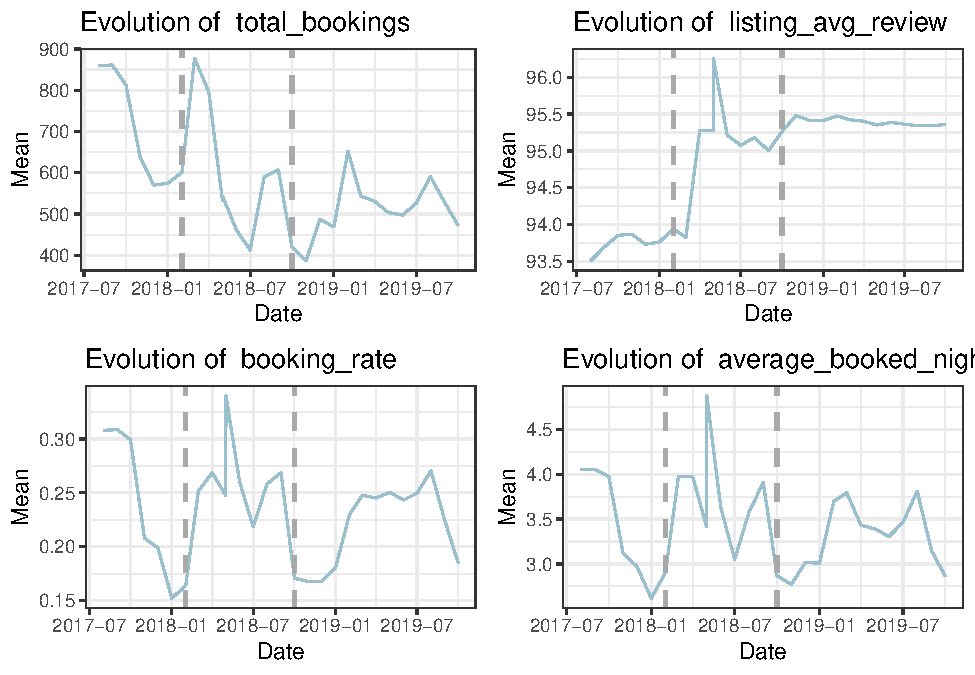
\includegraphics{Group-D---Assignment-1_files/figure-latex/unnamed-chunk-11-1.pdf}

Booking rate and average booked nights have a very similar performance
since they measure the same metric. The most notable insight is how the
implementation of the Plus program in San Francisco alone was able to
significantly increase these metrics. In the second implementation, said
metrics did see some performance increase but eventually dropped,
suggesting the Plus program was more of a success in San Francisco than
in the other cities. Listing average reviews had quite a volatile
performance, suggesting mixed results in the Plus program meeting
customer expectations. Later in other cities, reviews seemed to have
consistently increased showing an improvement in customer satisfaction.
Total bookings severely decreased after the Plus program in San
Francisco, indicating mixed results when compared to the positive
performance of booking rates. Perhaps, users booked more frequently but
also cancelled more often which can explain how total bookings dropped.
Later in other cities, total bookings also saw a consistent increase,
like booking rates and average reviews.

\textbf{Analysis of Booking Rate increase by city}

How much of the booking rate did the Plus program contribute to? Was it
more effective in San Francisco or in the later cities? In order to
answer these questions, we will compare this metric to those cities that
did not receive the Plus program at all.

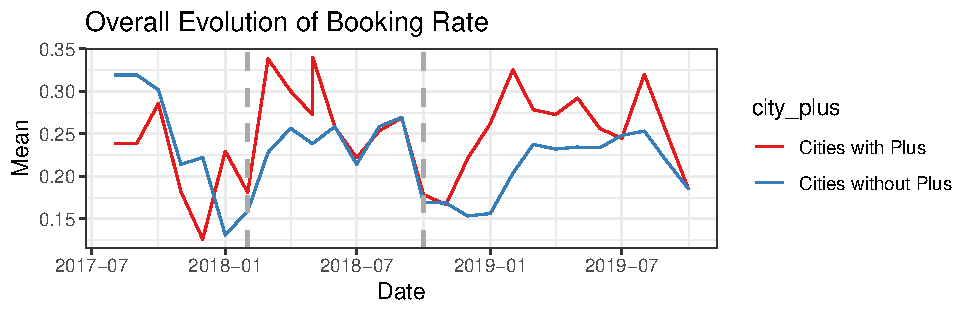
\includegraphics{Group-D---Assignment-1_files/figure-latex/unnamed-chunk-12-1.pdf}
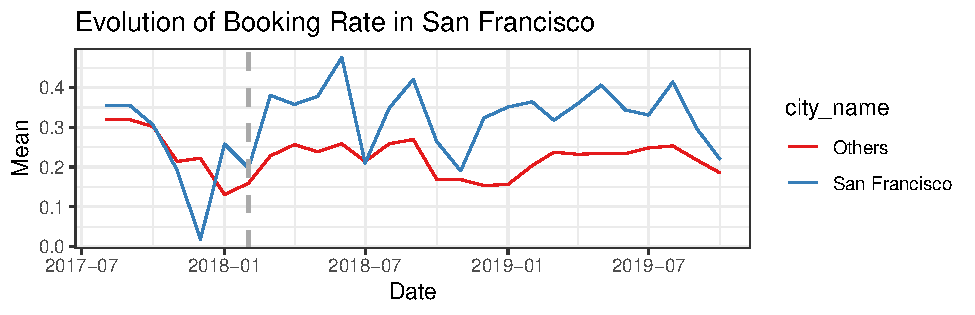
\includegraphics{Group-D---Assignment-1_files/figure-latex/unnamed-chunk-12-2.pdf}
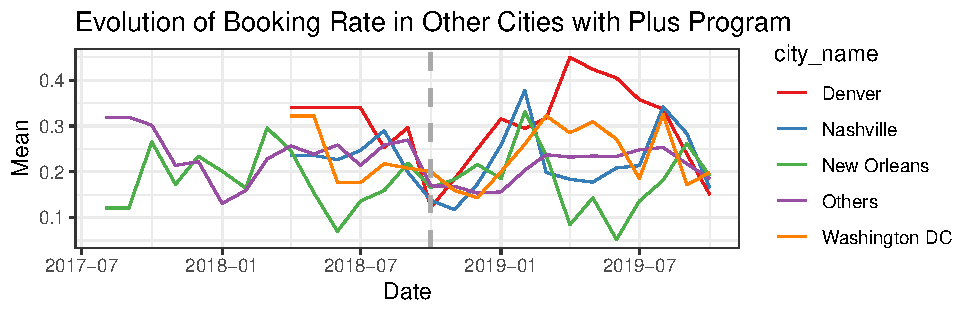
\includegraphics{Group-D---Assignment-1_files/figure-latex/unnamed-chunk-12-3.pdf}

The Plus program in San Francisco definitely increased booking rate
against cities that did not receive it. The program later implemented in
other cities (Denver, Nashville, New Orleans and Washington DC) also had
increased booking rates compared to all other cities. However, as it was
suggested in previous plots, the program in San Francisco seems to have
been more successful. It is possible that the Plus program in San
Francisco was more of a success because it was an unannounced pilot
program. The program in other cities could have been less of a success
for a large variety of reasons.

\textbf{Analysis of Average Rating in second stage cities}

If booking rates in the cities that got the Plus program (excluding San
Francisco) didn't see much of an increase, did they at least have better
average ratings, resulting in improved customer satisfaction?

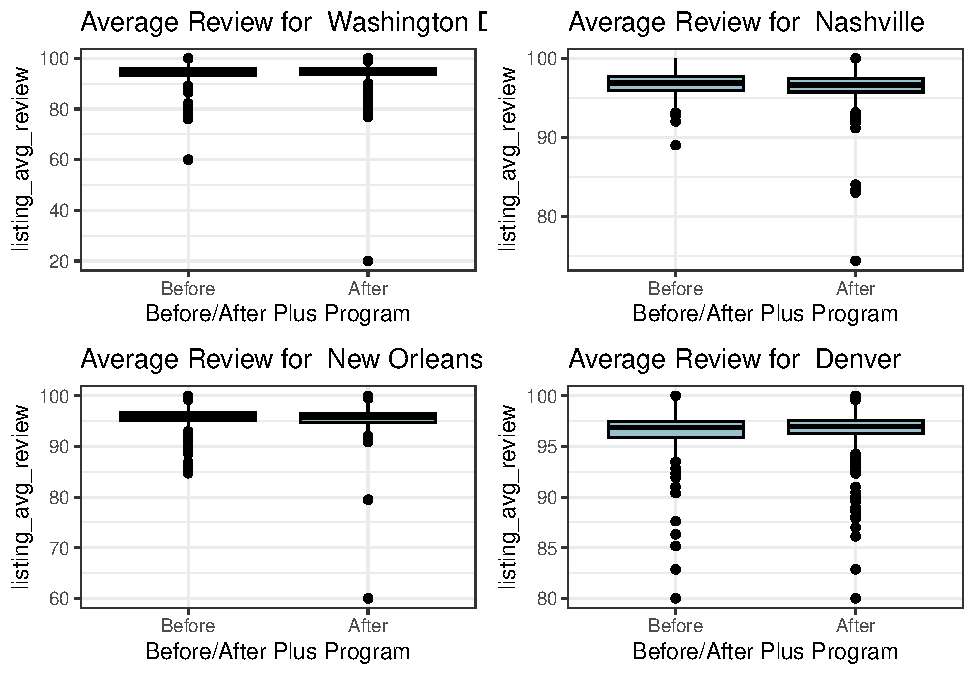
\includegraphics{Group-D---Assignment-1_files/figure-latex/unnamed-chunk-13-1.pdf}

Interestingly, the average rating in Washington DC, Nashville, New
Orleans and Denver didn't change that much. The average rating was
already very high. Perhaps, the Plus program in these cities did meet
customers' expectations which allowed the rating to stay consistently
high.

To recap, the assumptions we can extrapolate from the previous visual
inspections are the following: \textbf{overall booking rates increased
in cities after receiving the Plus program}; however, this same metric
\textbf{does not seem to have significantly improved in Denver,
Nashville, New Orleans, and Washington DC}; finally, in these cities the
\textbf{average review also seems to remain unchanged}.

\section{4. Hypothesis Testing}\label{hypothesis-testing}

To test the assumptions above, a short series of hypothesis testing will
be conducted. However, because there have been two implementations of
the Plus program, comparing the booking rate means of the Plus cities
before and after at different time periods introduces bias, since there
is mixed data between the two implementations. For this reason, the
means of all the booking rates will be \textbf{grouped by policy entry}
(whether the Plus program was present or not), instead of by time
period, to still determine before and after effects.

The first hypothesis is, therefore, the following:

\begin{itemize}
\item
  \(H_0:\) The booking rate mean before Plus implementation is equal or
  larger than that after implementation.
\item
  \(H_a:\) The booking rate mean before Plus implementation is smaller
  than that after implementation.
\end{itemize}

In order to test this hypothesis a left-tailed t-test will be conducted.

\begin{longtable}[]{@{}rrr@{}}
\toprule\noalign{}
policy\_entry & Mean & SD \\
\midrule\noalign{}
\endhead
\bottomrule\noalign{}
\endlastfoot
0 & 0.24 & 0.16 \\
1 & 0.26 & 0.18 \\
\end{longtable}

\begin{longtable}[]{@{}
  >{\raggedleft\arraybackslash}p{(\columnwidth - 12\tabcolsep) * \real{0.1429}}
  >{\raggedleft\arraybackslash}p{(\columnwidth - 12\tabcolsep) * \real{0.1286}}
  >{\raggedleft\arraybackslash}p{(\columnwidth - 12\tabcolsep) * \real{0.1143}}
  >{\raggedright\arraybackslash}p{(\columnwidth - 12\tabcolsep) * \real{0.1714}}
  >{\raggedleft\arraybackslash}p{(\columnwidth - 12\tabcolsep) * \real{0.1571}}
  >{\raggedleft\arraybackslash}p{(\columnwidth - 12\tabcolsep) * \real{0.1286}}
  >{\raggedleft\arraybackslash}p{(\columnwidth - 12\tabcolsep) * \real{0.1571}}@{}}
\toprule\noalign{}
\begin{minipage}[b]{\linewidth}\raggedleft
statistic
\end{minipage} & \begin{minipage}[b]{\linewidth}\raggedleft
t\_df
\end{minipage} & \begin{minipage}[b]{\linewidth}\raggedleft
p\_value
\end{minipage} & \begin{minipage}[b]{\linewidth}\raggedright
alternative
\end{minipage} & \begin{minipage}[b]{\linewidth}\raggedleft
estimate
\end{minipage} & \begin{minipage}[b]{\linewidth}\raggedleft
lower\_ci
\end{minipage} & \begin{minipage}[b]{\linewidth}\raggedleft
upper\_ci
\end{minipage} \\
\midrule\noalign{}
\endhead
\bottomrule\noalign{}
\endlastfoot
-4.004542 & 2398.474 & 3.2e-05 & less & -0.0247803 & -Inf &
-0.0145979 \\
\end{longtable}

The p-value of the test is extremely small, close to 0. Thus, the
observed difference between the two group means is \textbf{statistically
significant} at a 95\% confidence level, leading to reject the null
hypothesis of equality of means (p\textless0.05).

The second hypothesis will test the \textbf{strength of the
relationship} between booking rates and the implementation of the Plus
program in Denver, Nashville, New Orleans and Washington DC.

\begin{itemize}
\item
  \(H_0:\) There is no significant relationship between the booking rate
  and the implementation of the Plus program. \emph{(β1 = 0)}
\item
  \(H_a:\) There is a significant relationship between the booking rate
  and the implementation of the Plus program. \emph{(β1 ≠ 0)}
\end{itemize}

In order to test this hypothesis a linear regression model will be
applied.

\begin{longtable}[]{@{}lrr@{}}
\toprule\noalign{}
plus & Mean & SD \\
\midrule\noalign{}
\endhead
\bottomrule\noalign{}
\endlastfoot
After & 0.24 & 0.19 \\
Before & 0.24 & 0.15 \\
\end{longtable}

\begin{table}[!htbp] \centering 
  \caption{Relation Between Booking Rate and Plus Program} 
  \label{} 
\begin{tabular}{@{\extracolsep{5pt}}lc} 
\\[-1.8ex]\hline 
\hline \\[-1.8ex] 
 & \multicolumn{1}{c}{\textit{Dependent variable:}} \\ 
\cline{2-2} 
\\[-1.8ex] & booking\_rate \\ 
\hline \\[-1.8ex] 
 plusBefore & $-$0.002 \\ 
  & (0.007) \\ 
  Constant & 0.240$^{***}$ \\ 
  & (0.004) \\ 
 \hline \\[-1.8ex] 
Observations & 2,538 \\ 
R$^{2}$ & 0.00004 \\ 
Residual Std. Error & 0.177 (df = 2536) \\ 
\hline 
\hline \\[-1.8ex] 
\textit{Note:}  & \multicolumn{1}{r}{$^{*}$p$<$0.1; $^{**}$p$<$0.05; $^{***}$p$<$0.01} \\ 
\end{tabular} 
\end{table}

Even though β1 ≠ 0 (-0.0023), the p-value for this coefficient is
greater than 0.05. At a 95\% confidence level, the coefficient is
\textbf{not statistically significant}, indicating not enough
statistical evidence that there is a significant relationship between
the two variables.

Finally, the third hypothesis states the following:

\begin{itemize}
\item
  \(H_0:\) The average review mean for the second stage cities is equal
  before and after the plus implementation.
\item
  \(H_1:\) The average review mean for the second stage cities is
  different before and after the plus implementation.
\end{itemize}

In order to test this hypothesis a two-tailed t-test will be conducted.

\begin{longtable}[]{@{}rrr@{}}
\toprule\noalign{}
policy\_entry & Mean & SD \\
\midrule\noalign{}
\endhead
\bottomrule\noalign{}
\endlastfoot
0 & 95.55 & 3.51 \\
1 & 95.66 & 3.59 \\
\end{longtable}

\begin{longtable}[]{@{}
  >{\raggedleft\arraybackslash}p{(\columnwidth - 12\tabcolsep) * \real{0.1486}}
  >{\raggedleft\arraybackslash}p{(\columnwidth - 12\tabcolsep) * \real{0.1216}}
  >{\raggedleft\arraybackslash}p{(\columnwidth - 12\tabcolsep) * \real{0.1351}}
  >{\raggedright\arraybackslash}p{(\columnwidth - 12\tabcolsep) * \real{0.1622}}
  >{\raggedleft\arraybackslash}p{(\columnwidth - 12\tabcolsep) * \real{0.1486}}
  >{\raggedleft\arraybackslash}p{(\columnwidth - 12\tabcolsep) * \real{0.1486}}
  >{\raggedleft\arraybackslash}p{(\columnwidth - 12\tabcolsep) * \real{0.1351}}@{}}
\toprule\noalign{}
\begin{minipage}[b]{\linewidth}\raggedleft
statistic
\end{minipage} & \begin{minipage}[b]{\linewidth}\raggedleft
t\_df
\end{minipage} & \begin{minipage}[b]{\linewidth}\raggedleft
p\_value
\end{minipage} & \begin{minipage}[b]{\linewidth}\raggedright
alternative
\end{minipage} & \begin{minipage}[b]{\linewidth}\raggedleft
estimate
\end{minipage} & \begin{minipage}[b]{\linewidth}\raggedleft
lower\_ci
\end{minipage} & \begin{minipage}[b]{\linewidth}\raggedleft
upper\_ci
\end{minipage} \\
\midrule\noalign{}
\endhead
\bottomrule\noalign{}
\endlastfoot
-0.7300316 & 1878.441 & 0.4654619 & two.sided & -0.1072067 & -0.3952171
& 0.1808038 \\
\end{longtable}

The p-value of the test is greater than 0.05. So at a 95\% confidence
level, there is \textbf{no evidence of significant difference} between
the means, leading to fail to reject the null hypothesis of equality of
means.

\section{Conclusion}\label{conclusion}

In conclusion, it can be deduced that overall \textbf{booking rates
significantly improved} after implementing the Plus program. It was
found that the difference between the booking rate means was
statistically significant.

But, the change in \textbf{booking rate means was different} between the
first implementation of the Plus program in San Francisco and the second
in Nashville, New Orleans, Washington DC and Denver.

The first program in San Francisco seems much more successful, perhaps
because it was essentially an unannounced pilot program. Therefore, it
was worth investigating the effect of the program specifically in
Nashville, New Orleans, Washington DC and Denver. Interestingly,
\textbf{no evidence of a significant relationship was found between the
implementation of Plus program and increase in booking rates}.

Since the Plus program seemed to be less of a success in these cities
when compared to San Francisco, it was worth exploring whether customer
satisfaction changed instead. After testing for it, it was shown that
there is \textbf{not enough evidence to conclude that there is a
difference between means of listing average reviews}.

In other words, the Plus program increased overall booking rates. The
Plus program in San Francisco was a success, although it was a pilot
one. In the cities where the program was later implemented, there was no
relationship between the booking rates and the implementation of the
program. Customer satisfaction might have played a role, except that no
significant difference was found. This analysis was insightful to
suggest several demographic topics for further research. Why was the
pilot program such a success? Did employment rate play a role? Perhaps,
San Francisco is a larger CBD than other cities, leading to better
match-making for premium accommodations. Did seasonality matter during
the second implementation? It could be that the program was less of a
success since it was introduced after Summer, a time where people
generally come back from holidays and book less vacations.

\vspace{60pt}

\textbf{Disclaimer}

This research paper had its code deliberately debugged with the help of
AI, making sure that the inevitable human errors were swiftly corrected
by our digital assistant. Rest assured, no robots were harmed in the
process, and the human touch remained essential. Other than debugging,
AI was also used for coding suggestions and alternatives.

\emph{Fun fact:} this disclaimer was written by AI

\end{document}
